\section{Базовый алгоритм}
Базовым алгоритмом в данной задаче является метод частичных наименьших квадратов (далее PLS).
Метод PLS относится к классу методов проекции на подпространства, которые предполагают поиск собственного базиса с последующим выбором в нем некоторого количества собственных векторов. Другие методы проекции на подпространства включают в себя метод главных компонент, линейный дискриминантный анализ и канонический корреляционный анализ. 

Метод PLS выгодно отличает то, что он позволяет одновременно выявлять скрытые связи между входными данными и аппроксимировать их. Более того, существуют реализации метода PLS, позволяющие построить регрессионную модель, описывающую зависимость между входными данными. 
Метод  PLS позволяет выделить из исходных данных компоненты, между которыми существует ковариационная связь. На основе этих компонент может быть построена модель регрессии. Такой подход позволяет не только существенно снизить вычислительные затраты, но и значительно улучшить точность модели по сравнению с линейной регрессией, построенной с помощью метода наименьших квадратов. 

\section{Метрики}
Для оценки качества предсказания использовались метрики mean squared error, mean absolute error и r2 score:
\[
  mse = \frac1n \sum_{i = 1}^n (y_i - \hat{y}_i)^2 \]\[
  mae = \frac1n \sum_{i = 1}^n |y_i - \hat{y}_i| \]\[
  r2 = 1 - \frac{\sum_{i = 1}^n (y_i - \hat{y}_i)^2}{\sum_{i = 1}^n (y_i - \overline{y})^2}
\]
Здесь $y_i$~--- предсказываемые данные, $\hat{y}_i$~--- предсказание модели, $\overline{y} = \frac1n \sum_{i = 1}^n y_i$~--- среднее $y_i$.

\section{Базовый эксперимент}
Для проведения эксперимента, из данных электрокортикограммы были выделены частоты сигналов. Выходные данные~--- трехмерные координаты движения руки обезьяны. Полученные данные были разделены на обучающую и контрульную выборки в отношении два к одному. На полученной выборке был обучен PLS с различным количеством компонент (от 2 до 100). Результаты эксперимента представлены на рис.~\ref{fig:baseAlgo}.
\begin{figure}
  \begin{center}
    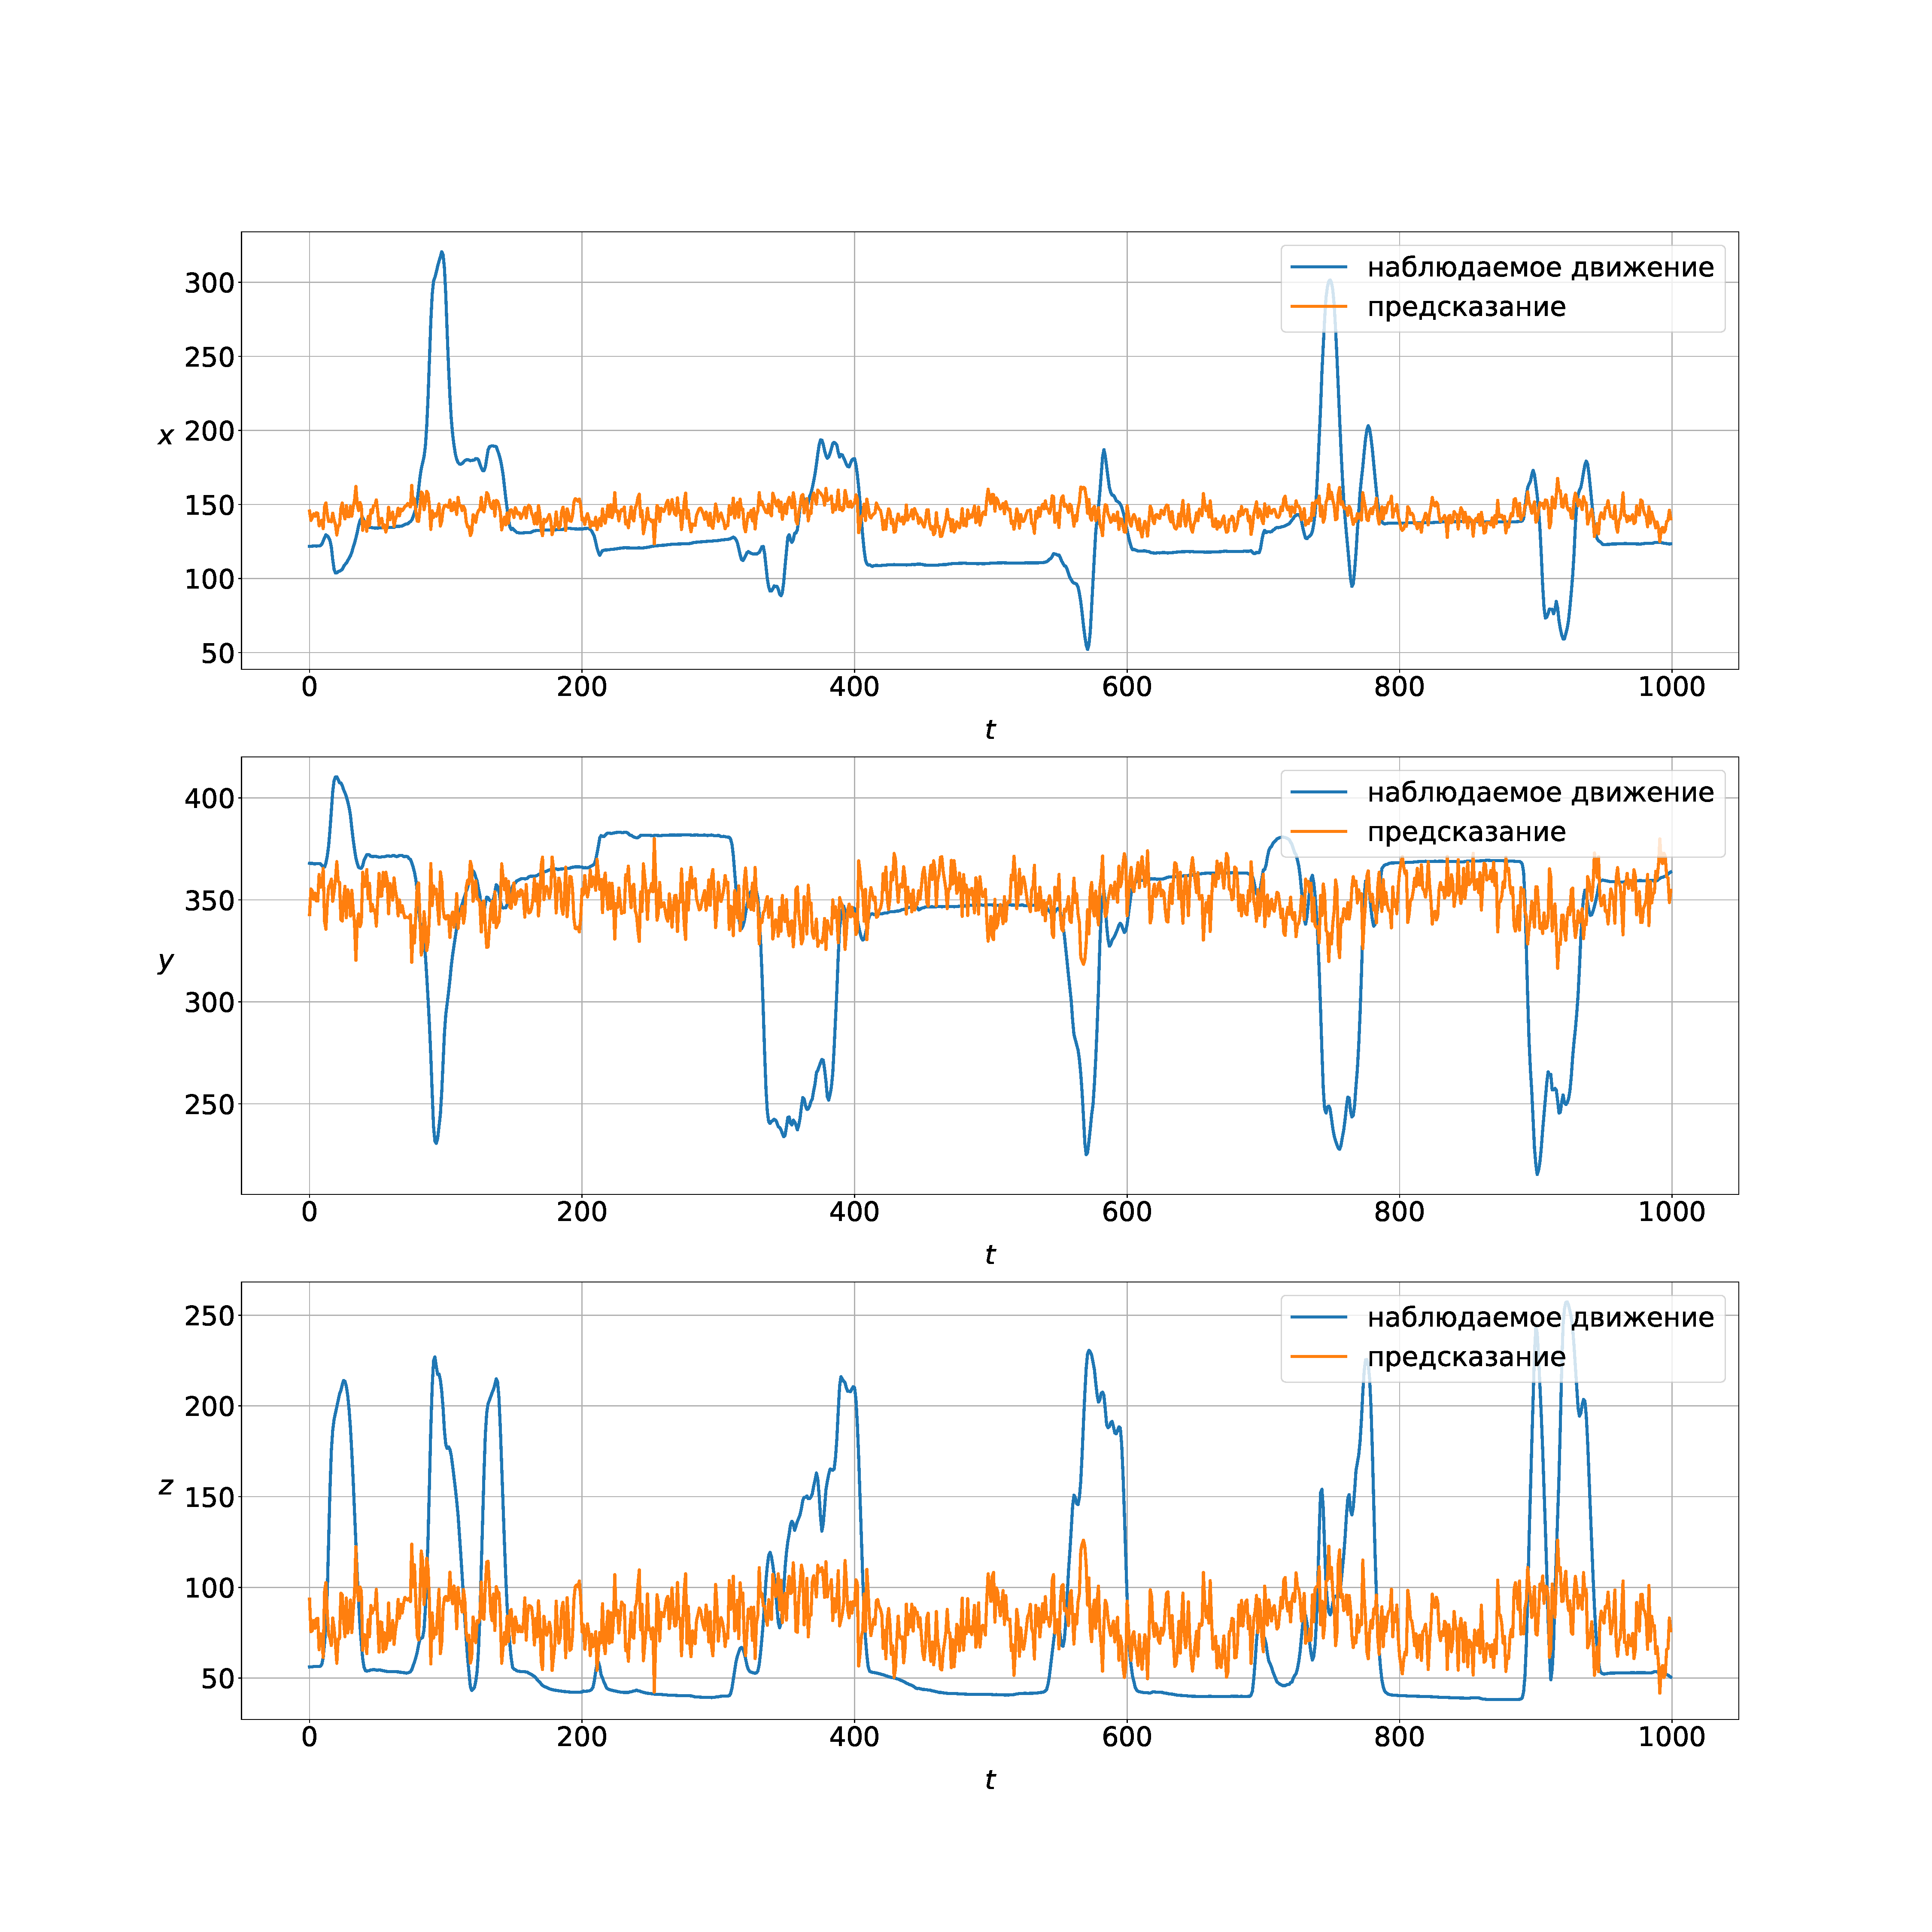
\includegraphics[width=\textwidth]{base_algo.pdf}
    \caption{Предсказания двухкомпонентного PLS, обученного на исходных данных}
    \label{fig:baseAlgo}
  \end{center}
\end{figure}
На графике представлена зависимость координаты конечности от времени. Как видно из рисунка, базовый алгоритм довольно плохо справляется с поставленной задачей. Общий профиль пиков соблюдается, однако PLS очень грубо оценивает острые пики. Также предсказание испытывает флуктуации, когда конечность почти не движется. В результате погрешность предсказания высока. Эксперимент показал значения метрик $mae = 30.17, mse = 1843.91, r2 = 0.01$. Для борьбы с погрешностями предлагается снизить размерность входного сигнала.
